\documentclass[a4paper, 12pt]{article}
\usepackage{graphicx}
\usepackage[margin=2cm]{geometry}
\usepackage[hidelinks]{hyperref}
\usepackage[croatian]{babel}
\usepackage[sorting=none]{biblatex}
    \addbibresource{ref.bib}
\usepackage{float}


% Boje za kod:
\usepackage{xcolor,graphicx}
\usepackage{listings}

\definecolor{solarized-base03}{RGB}{0, 43, 54}
\definecolor{solarized-base02}{RGB}{7, 54, 66}
\definecolor{solarized-base01}{RGB}{88, 110, 117}
\definecolor{solarized-base00}{RGB}{101, 123, 131}
\definecolor{solarized-base0}{RGB}{131, 148, 150}
\definecolor{solarized-base1}{RGB}{147, 161, 161}
\definecolor{solarized-base2}{RGB}{238, 232, 213}
\definecolor{solarized-base3}{RGB}{253, 246, 227}
\definecolor{solarized-yellow}{RGB}{181, 137, 0}
\definecolor{solarized-orange}{RGB}{203, 75, 22}
\definecolor{solarized-red}{RGB}{220, 50, 47}
\definecolor{solarized-magenta}{RGB}{211, 54, 130}
\definecolor{solarized-violet}{RGB}{108, 113, 196}
\definecolor{solarized-blue}{RGB}{38, 139, 210}
\definecolor{solarized-cyan}{RGB}{42, 161, 198}
\definecolor{solarized-green}{RGB}{133, 153, 0}

\lstset{
  basicstyle=\footnotesize\ttfamily\color{solarized-base00},
  keywordstyle=\color{solarized-blue}\bfseries,
  commentstyle=\color{solarized-base1},
  stringstyle=\color{solarized-cyan},
  identifierstyle=\color{solarized-violet},
  numberstyle=\tiny\color{solarized-base01},
  numbers=left,
  firstnumber=1,
  stepnumber=1,
  showstringspaces=false,
  tabsize=4,
  frame=none,
  framerule=1pt,
  framexleftmargin=5pt,
  framexrightmargin=5pt,
  framextopmargin=3pt,
  framexbottommargin=3pt,
  backgroundcolor=\color{solarized-base3},
  rulecolor=\color{solarized-base01},
  breaklines=true,
  breakatwhitespace=true,
  language=C++
}


\begin{document}
\noindent
Univerzitet u Sarajevu\\
Elektrotehnički fakultet\\
Predmet: Uvod u digitalnu obradu slike\\
Predmetni profesor: prof. dr Emir Sokić\\
Autor: Berina Biberović\\
Akademska godina: 2022/2023.


\begin{center}
    \section*{Tutorijal 5}
    \subsection*{Operacije nad slikama u frekventnom domenu. \textit{Deblur}.}
\end{center}

Ovaj tutorijal će da bude uputstvo za laboratorijsku vježbu 5 koja se bavi \textit{deblur} efektom nad slikama, zbog toga što je primjećeno da laboratorijska vježba 5 predstavlja veliki problem studentima prilikom izrade.

Kod priložen u tutorijalu je zasnovan na kodu sa \href{https://docs.opencv.org/3.4/d1/dfd/tutorial_motion_deblur_filter.html}{linka}. Autor je morao napraviti izmjene kako bi se dobili željeni rezultati, zbog čega se korišteni kod nalazi ispod. Pretpostavka je da je \textit{blur} koji je nastao na slici posljedica linearnog kretanja.

\begin{lstlisting}
#include <string>
#include <opencv4/opencv2/imgproc.hpp>
#include <opencv4/opencv2/highgui.hpp>
#include <opencv4/opencv2/core/mat.hpp>
#include <opencv4/opencv2/imgcodecs.hpp>
#include <opencv4/opencv2/core/matx.hpp>


// Odabrati jednu od funkcija.
void calcPSF(cv::Mat& outputImg, cv::Size filterSize, int len, double theta) {	// Linear motion
    cv::Mat h(filterSize, CV_32F, cv::Scalar(0));
    cv::Point point(filterSize.width / 2, filterSize.height / 2);
    cv::ellipse(h, point, cv::Size(0, cvRound(float(len) / 2.0)), 90.0 - theta, 0, 360, cv::Scalar(255), cv::FILLED);
    cv::Scalar summa = sum(h);
    cv::namedWindow("FILTER", cv::WINDOW_NORMAL);
    imshow("FILTER", h);
    outputImg = h / summa[0];
}


// Pogledati https://docs.opencv.org/4.x/d8/d01/tutorial_discrete_fourier_transform.html
void fftshift(const cv::Mat& inputImg, cv::Mat& outputImg) {
    outputImg = inputImg.clone();
    int cx = outputImg.cols / 2;
    int cy = outputImg.rows / 2;
    cv::Mat q0(outputImg, cv::Rect(0, 0, cx, cy));
    cv::Mat q1(outputImg, cv::Rect(cx, 0, cx, cy));
    cv::Mat q2(outputImg, cv::Rect(0, cy, cx, cy));
    cv::Mat q3(outputImg, cv::Rect(cx, cy, cx, cy));
    cv::Mat tmp;
    q0.copyTo(tmp);
    q3.copyTo(q0);
    tmp.copyTo(q3);
    q1.copyTo(tmp);
    q2.copyTo(q1);
    tmp.copyTo(q2);
}

void filter2DFreq(const cv::Mat& inputImg, cv::Mat& outputImg, const cv::Mat& H) {
    cv::Mat planes[2] = { cv::Mat_<float>(inputImg.clone()), cv::Mat::zeros(inputImg.size(), CV_32F) };
    cv::Mat complexI;
    merge(planes, 2, complexI);
    dft(complexI, complexI, cv::DFT_SCALE);
    cv::Mat planesH[2] = { cv::Mat_<float>(H.clone()), cv::Mat::zeros(H.size(), CV_32F) };
    cv::Mat complexH;
    cv::merge(planesH, 2, complexH);
    cv::Mat complexIH;
    cv::mulSpectrums(complexI, complexH, complexIH, 0);
    cv::idft(complexIH, complexIH);
    cv::split(complexIH, planes);
    outputImg = planes[0];
}

void calcWnrFilter(const cv::Mat& input_h_PSF, cv::Mat& output_G, double nsr) {
    cv::Mat h_PSF_shifted;
    fftshift(input_h_PSF, h_PSF_shifted);
    cv::Mat planes[2] = { cv::Mat_<float>(h_PSF_shifted.clone()), cv::Mat::zeros(h_PSF_shifted.size(), CV_32F) };
    cv::Mat complexI;
    cv::merge(planes, 2, complexI);
    cv::dft(complexI, complexI);
    cv::split(complexI, planes);
    cv::Mat denom;
    pow(abs(planes[0]), 2, denom);
    denom += nsr;
    cv::divide(planes[0], denom, output_G);
};

void edgetaper(const cv::Mat& inputImg, cv::Mat& outputImg, double gamma, double beta) {
    int Nx = inputImg.cols;
    int Ny = inputImg.rows;
    cv::Mat w1(1, Nx, CV_32F, cv::Scalar(0));
    cv::Mat w2(Ny, 1, CV_32F, cv::Scalar(0));
    float* p1 = w1.ptr<float>(0);
    float* p2 = w2.ptr<float>(0);
    float dx = float(2.0 * CV_PI / Nx);
    float x = float(-CV_PI);
    for (int i = 0; i < Nx; i++) {
        p1[i] = float(0.5 * (tanh((x + gamma / 2) / beta) - tanh((x - gamma / 2) / beta)));
        x += dx;
    }
    float dy = float(2.0 * CV_PI / Ny);
    float y = float(-CV_PI);
    for (int i = 0; i < Ny; i++) {
        p2[i] = float(0.5 * (tanh((y + gamma / 2) / beta) - tanh((y - gamma / 2) / beta)));
        y += dy;
    }
    cv::Mat w = w2 * w1;
    cv::multiply(inputImg, w, outputImg);
}

int main(){
    std::string ime = "slika.jpeg";
    cv::Mat slika;
    slika = imread("../" + ime, cv::IMREAD_GRAYSCALE);

    cv::Mat rezultat;

    // Srezati sliku na paran broj redova i kolona
    cv::Rect roi = cv::Rect(0, 0, slika.cols & -2, slika.rows & -2);

    // Racunanje Wienerovog filtera
    cv::Mat Hw, h;

    cv::namedWindow("Trackbars", cv::WINDOW_NORMAL);
    cv::namedWindow("Izlaz", cv::WINDOW_NORMAL);

    cv::createTrackbar("t1", "Trackbars", nullptr, 500);
    cv::createTrackbar("t2", "Trackbars", nullptr, 180);
    cv::createTrackbar("t3", "Trackbars", nullptr, 1000);

    char keyPress;
    cv::Mat pomocna;
    while(true) {
        
        int t1 = cv::getTrackbarPos("t1", "Trackbars");
        int t2 = cv::getTrackbarPos("t2", "Trackbars");
        int t3 = cv::getTrackbarPos("t3", "Trackbars");

        calcPSF(h, roi.size(), t1, t2);
        calcWnrFilter(h, Hw, 1.0 / double(t3));

        slika.convertTo(slika, CV_32F);

        edgetaper(slika, pomocna, 10, 10);

        // Filtriranje
        filter2DFreq(pomocna(roi), rezultat, Hw);

        // Prikazivanje filtrirane slike
        rezultat.convertTo(rezultat, CV_8U);
        cv::normalize(rezultat, rezultat, 0, 255, cv::NORM_MINMAX);
        cv::imshow("Izlaz", rezultat);

        if(cv::waitKey() == 'q') break;
    }

    cv::imwrite("../Rezultat.jpeg", rezultat);
    return 0;
}
\end{lstlisting}

U gornjem kodu možemo primijetiti da smo napravili 5 \textit{user defined} funkcija: \lstinline{calcPSF}, \lstinline{fftshift}, \lstinline{filter2DFreq}, \lstinline{calcWnrFilter} i \lstinline{edgetaper}. Sve ove funkcije će biti objašnjene kako budemo prolazili kroz \lstinline{main} funkciju.

Unutar \lstinline{main} funkcije učitavamo \textit{grayscale} sliku nad kojom želimo da maknemo mućenje (eng. \textit{blur}). Nakon toga korištenjem konstruktora klase \lstinline{cv::Rect} ćemo srezati sliku na paran broj redova i kolona - rezultat toga stavljamo u objekat istog tipa. Naravno, imenujemo odgovarajuće instance klase \lstinline{cv::Mat} koje će nam kasnije trebati - \lstinline{rezultat}, \lstinline{Hw}, \lstinline{pomocna} i \lstinline{h}.

Onda pravimo tri \textit{trackbar}-ove uz pomoć kojih ćemo sklanjati uticaj mućenja sa slike, što će detaljno biti u nastavku objašnjeno. Ulaskom u \lstinline{while} petlju, prvo uzimamo vrijednosti tri varijable \lstinline{t1}, \lstinline{t2} i \lstinline{t3} za koje smo napravili prethodno \textit{trackbar}-ove. 

Pozivamo onda funkciju \lstinline{calcPSF} kojoj prosljeđujemo \lstinline{h}, veličinu varijable \lstinline{roi}, \lstinline{t1} i \lstinline{t2}. Ova funkcija služi da se uz pomoć \textit{linear motion}-a dobije slika kretanja. Detaljno možete o ovome pročitati na \href{https://docs.opencv.org/4.x/d1/dfd/tutorial_motion_deblur_filter.html}{linku}. 

Nakon toga pozivamo funkciju \lstinline{calcWnrFilter} koja računa Wienerov filter. Prosljeđujemo joj varijable \lstinline{h}, \lstinline{Hw}, \lstinline{1.0 / t3}. Ključan aspekt za primjenu Wienerovog filtera za pokušaj uklanjanja šuma sa slike je precizno definisanje kretanja objekata na slici. U ovu svrhu koristimo \textit{point spread} funkciju, koja definiše kako se jedna tačka pomjerila za vrijeme otvora blende kamere pri pravljenju fotografije. Pri pokretanju programa potrebno je uskladiti ovu funkciju sa kretanjem u prostoru slike korištenjem parametara \lstinline{len} i \lstinline{theta} (koji odgovaraju količini kretanja jednog piksela u području od interesa i ugao u ravni slike). Pored ovoga porebno je odrediti SNR radi primjene Wienerovog filtra.

Ključna pretpostavka je da je kretanje svake tačke u ravni slike identično. Naravno, ovo nije valjana pretpostavka uvijek, ali se može pretpostaviti da je tačna lokalno, čime se omogućuje \textit{deblur} efekat objekta ili dijela slike od interesa. Kako se u idealnom slučaju šum uslijed kretanja manifestuje kao konvolucija slike sa binarnom slikom koja sadrži liniju koja predstavlja kretanje jedne svake tačke u slici tako je \textit{deblur} zapravo problem dekonvolucije. Wienerova dekonvolucija koristi upravo Wienerov filter kako bi se uklonio šum. 

Vrijedno spomena je da njegova direktna primjena dolazi do problema pri ivici slike, pošto je potrebna informacija o slici van okvira slike, što dovodi do tzv. \textit{ringing} efekta. Uslijed digitalne prirode slike dolazi do nepovratnog gubitka informacija zbog čega je nerazumno očekivati od bilo kakve metode da uradi savršen \textit{debluring}, no \textit{debluring} metode mogu itekako pomoći u povratku dijela kvaliteta slike. Da bismo što više mogli umanjiti \textit{ringing} efekat, korištena je za to funkcija \lstinline{edgetaper} koja prima u prethodnoj liniji konvertovanu sliku u tip \lstinline{CV_32F}, spašava rezultat funkcije u varijablu \lstinline{pomocna} i prima dva parametra \lstinline{gamma} i \lstinline{beta} koji služe za transformaciju piksela na rubu slike.

Nakon toga se poziva funkcija \lstinline{filter2DFreq} koja prima ulaznu sliku \lstinline{pomocna(roi)}, vraća izlaznu sliku \lstinline{rezultat} i prima matricu \lstinline{Hw} koju smo dobili iz funkcije \lstinline{calcWnrFilter}. \lstinline{rezultat} se onda konvertuje u tip \lstinline{CV_8U}, normalizira se i na ekranu pokazujemo izgled slike nakon primjenjivanja svih ovih filtera na njega. 

Za funkciju \lstinline{fftshift} koja radi \textit{shift}-anje u 2D-u, možete detaljnije pročitati na \href{https://docs.opencv.org/4.x/d8/d01/tutorial_discrete_fourier_transform.html}{linku}.

Originalna slika koja je ubačena u filter je prikazana na slici \ref{sl1}. Rezultat nakon filtriranja koji je prikazan na slici \ref{sl2} je dobiven za parametre \lstinline{t1 = 18}, \lstinline{t2 = 11} i \lstinline{t3 = 48} za datu sliku.

\begin{figure}[H]
    \minipage{0.49\textwidth}
        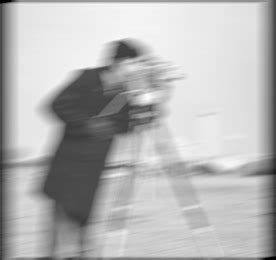
\includegraphics[width=\linewidth]{Slike/slika.jpeg}
        \caption{Originalna slika}\label{sl1}
    \endminipage\hfill
    \minipage{0.49\textwidth}
        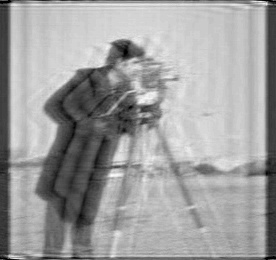
\includegraphics[width=\linewidth]{Slike/Rezultat.jpeg}
        \caption{Rezultat nakon \textit{debluring}-a}\label{sl2}
    \endminipage\hfill
\end{figure}

\subsection*{Napomene}

Korištena tema za prikaz C++ koda na tutorijalima je \href{https://ethanschoonover.com/solarized/}{\lstinline{solarized}}\cite{solarized}.

\printbibliography


\end{document}
